\documentclass[11pt] {article}
\usepackage{graphicx}
\usepackage{listings}

\begin{document}
\vspace{10mm} %5mm vertical space
$$
\includegraphics[scale = 4]{alatoo}$$

\begin{center}
{\Huge LIMITS IN PYTHON \par}
\end{center}

\vspace{70mm} %5mm vertical space
\hfill Name: S.Betul Polat

\hfill Course Name: Calculus

\hfill Group: COM-18



\vspace{500mm} %5mm vertical space
\begin{center}
ACKNOWLEDGEMENT
\end{center}
First of all I would like to thank our lecturer Tahir Aslan for supporting  us in learning the Calculus and for supporting us when we need help.

Beside from my lecturer, I like to thank other students for their effort.
 
Completing their report and for carrying the spirit of solidarity. 

We, the students, believe that we will be successful citizens and educators if we receive the necessary education to guarantee our future.

In order to accomplish some things, it is necessary to work hard and make efforts. 

We need an environment where we can work hard to survive the challenges and go on new and bright days, and we need supporters who trust us. 

But success starts with self-confidence, so first of all thanks to our family and friends and of course our teachers.


\vspace{150mm} %5mm vertical space
\begin{center}
INTRODUCTION

Python programming language is a highly preferred language. 

And it has a mass of people dedicated to self-improvement.

It is a language that is very similar to Java language and has a practical use. 

It also allows to solve many mathematical operations. 

Our successful programmers have developed many applications so that we can perform such operations. 

For example, I can give examples with limits. 

Instead of solving it ourselves, we can create graphics with these programs and then enable any desired process to go into function.

We have been given many opportunities to improve ourselves and adapting such programming languages 

in short, within the learning strategy in computer programming languages, makes our life easier. 

And the python programming language allows you to practically pour many operations in code into mathematics
\end{center}

\vspace{150mm} %5mm vertical space
\begin{center}
EXPLANATIONS

Installation Steps:

1.	Install Anaconda, link - https://www.anaconda.com/distribution/ 

2.	Python if you prefer - https://www.python.org/downloads/

3.	Spyder without anaconda - https://www.spyder-ide.org/

4.	Jupyter - https://jupyter.org/install
\end{center}

\vspace{60mm} %50mm vertical space
\begin{center}
EXCECUTION PROCEDURES
\end{center}

\begin{center}
A small transaction about limit is an example where we pass the values given to us with python. 

Presented the answer as 2
\end{center}

\begin{lstlisting}[language=Python]
from sympy import *
x = symbols('x')
expr = (x**2-1)/(x-1);
limit_expr = limit(expr, x,1)
print("limit of the expression: {}".format(limit_expr))
\end{lstlisting}

\begin{center}
Result = limit of the expression: 2
\end{center}

\vspace{120mm} %5mm vertical space
\begin{center}
2. In our example, the transaction is made with the limit. And in this process, we can additionally see the graph
\end{center}

\begin{lstlisting}[language=Python]
import matplotlib.pyplot as plt
import numpy as np

x = symbols('x');
y = symbols('y');
expr = (x**2-1)/(x+1);
limit_expr = limit(expr, x,1)
print(limit_expr)
x = np.linspace(0,5)
y = x-1
plt.plot(x,y,'*', 'o')
plt.show()
\end{lstlisting}

\begin{center}
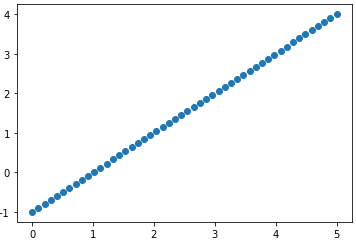
\includegraphics[scale = 1]{img2}
\end{center}

\vspace{150mm} %5mm vertical space
\begin{center}
Example 2 shows a python operation related to the limit. As it is known, we can make many examples like this.
\end{center}
\begin{lstlisting}[language=Python]
from sympy import * 
  
x = symbols('x') 
expr = sin(3 * x)/x; 
    
print("Expression : {}".format(expr))  
      
limit_expr = limit(expr, x, 0)   
      
print("Limit of the expression tends to 0 : {}".format(limit_expr))
\end{lstlisting}

\begin{center}
Result = Expression : sin(3*x)/x

Limit of the expression tends to 0 : 3
\end{center}

\vspace{150mm} %5mm vertical space
\begin{center}
In this example, a sample taken from the previous limit sample and obtained with a graph
\end{center}

\begin{lstlisting}[language=Python]
from sympy import * 
  
x = symbols('x') 
expr = sin(3 * x)/x; 
    
print("Expression : {}".format(expr))  
      
limit_expr = limit(expr, x, 0)   
      
print("Limit of the expression tends to 0 : {}".format(limit_expr))

k = np.linspace(3,6)  
x = np.linspace(0,6)
 
y = x**2
z = x-1
 
plt.plot(x,y,k,z)
  
plt.show() 
\end{lstlisting}

$$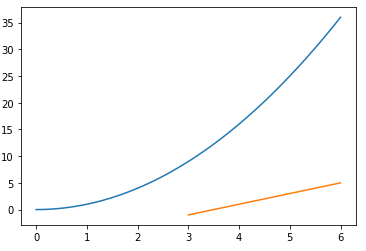
\includegraphics[scale = 1]{img3}$$
\vspace{15mm} %5mm vertical space
\begin{center}
CONCLUSION
\end{center}
Limit is a function of a calculus and considered as a fundamental concept

Helps to analysize the input or a function that we have given

Moreover a python code helps to implement, In addition to that  with the help of given methods

its simple and more practical to find the given instructions

which is called as limit in a mathematical way.
 

\vspace{160mm} %5mm vertical space
\begin{center}
REFERENCES

1.	https://medium.com/@mindfiresolutions.usa/python-7-important-reasons-why-you-should-use-python-5801a98a0d0b

2.	https://stackoverflow.com/questions/1792360/what-are-the-limits-of-python

3.	http://www.quantatrisk.com/2014/09/17/deriving-limits-in-python/
\end{center}
\end{document}
